\chapter{Developer Guidelines}
\label{DeveloperGuidelines}

CrypTool 2.0 is built upon state-of-the-art technologies such as .NET 4.0 and the Windows Presentation Foundation (WPF). Before you can start writing code and adding to the development of the project, a few things need to be considered. To make this process easier, please read through this document and follow the instructions closely. This document exists to help get you started by showing you how CrypTool 2 plugins are built in order to succesfully interact with the application core. We have tried to be very thorough, but if you encounter a problem or error that is not described here, please let us know. Not only do we want to help get you up and running, but we also want to add the appropriate information to this guide for the benefit of other future developers.

In this first chapter we will describe all steps necessary in order to compile CrypTool 2 on your own computer. This is always the first thing you need to do before you can begin developing your own plugins and extensions. The basic steps are:
\begin{itemize}
	\item Getting all prerequisites and installing them
	\item Accessing and downloading the source code with SVN
	\item Compiling the latest version of the source code
\end{itemize}

\section{Prerequisites}
\label{Prerequisites}

Since CrypTool 2 is based on Microsoft .NET 4.0, you will need a Microsoft Windows environment. (Currently no plans exist for porting this project to Mono or other platforms.) We have successfully tested with \textbf{Windows XP}, \textbf{Windows Vista} and \textbf{Windows 7}.

Since you are reading the developer guidelines, you probably want to develop something. Hence, you will need a development environment. In order to compile our sources you need \textbf{Microsoft Visual Studio 2010} or \textbf{Microsoft Visual C\# 2010 Express}. Make sure to always install the latest service packs for Visual Studio.

In order to run or compile our source code you will need at least the \textbf{Microsoft .NET 4.0}. Usually the installation of Visual Studio also installs the .NET framework, but if you do not have the latest version, you can get it for free from \href{http://www.microsoft.com/downloads/details.aspx?FamilyID=9cfb2d51-5ff4-4491-b0e5-b386f32c0992}{Microsoft's website}. Once the framework has been installed, your development environment should be ready for our source code.
\clearpage

\section{Accessing the Subversion (SVN) repository}
\label{AccessingSubversion}

Next you will need a way of accessing and downloading the source code. For the CrypTool 2 project we use \textbf{Subversion (SVN)} for version control, and hence you will need an SVN client, i.e.\ \textbf{TortoiseSVN}, \textbf{AnkhSVN} or the \textbf{svn commandline from cygwin}, to access our repository. It does not matter which client you use, but if SVN is new to you, we suggest using \href{http://www.tortoisesvn.net/}{TortoiseSVN}, since it offers a handy, straightforward Windows Explorer integration. We will guide you through how to use TortoiseSVN, although you should be able to use any SVN client in a similar fashion.

\subsection{Checking out the sources}
\label{CheckingOutTheSources}

First, download and install TortoiseSVN. This will require you to reboot your computer, but once it is back up and running, create a directory (for instance, \textit{CrypTool2}) somewhere on your computer for storing the local working files. Right-click on this directory; now that TortoiseSVN has been installed, you should see a few new items in the context menu (Figure~\ref{fig:tortoise_svn_checkout}). Select \textit{SVN Checkout}.

\begin{figure}[h!]
	\centering
		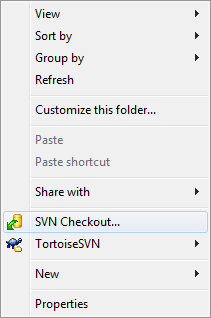
\includegraphics[width=0.40\textwidth]{figures/tortoise_svn_checkout.png}
	\caption{Selecting \textit{SVN Checkout} from the context menu after installing TortoiseSVN.}
	\label{fig:tortoise_svn_checkout}
\end{figure}
\clearpage

A window will now appear that will ask you for the URL of the repository that you would like to access. Our code repository is stored at \url{https://www.cryptool.org/svn/CrypTool2/trunk/}, and this is what you should enter in the appropriate field. The \textit{Checkout directory} should already be filled in correctly with your new folder, and you shouldn't need to change any other options.

\begin{figure}[h!]
	\centering
		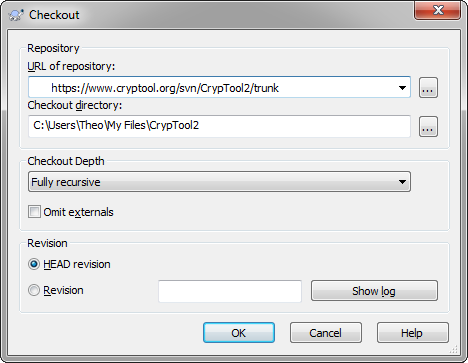
\includegraphics[width=0.60\textwidth]{figures/tortoise_svn_checkout_window.png}
	\caption{Checking out the CrypTool 2 repository.}
	\label{fig:tortoise_svn_checkout2}
\end{figure}

Then just hit \textit{OK}. You may be asked to accept a certificate (which you should accept), and you will certainly be asked for login information. You can use the \textit{anonymous} user with no password for readonly access. If you are a registered developer, you should have already been given a username and password, and you should enter them here. (These are the same username and password that you can use for the \href{https://www.cryptool.org/trac/CrypTool2/wiki}{CrypTool 2 development wiki}.) If you are a guest and just want to download the source code, you can use ``anonymous'' as the username and an empty password. Mark the checkbox for saving your credentials if you don't want to enter them every time you work with the repository (your password will be saved on your computer). Finally, hit \textit{OK}, and the whole CrypTool 2 repository will begin downloading into your chosen local directory.

Since CrypTool 2 is a collaborative project with many developers, changes are made to the repository rather frequently. You should maintain a current working copy of the files to ensure your interoperability with the rest of the project, and thus you should update to the latest version as often as possible. You can do this by right-clicking on any directory within the working files and choosing \textit{SVN~Update} from the context menu.

A TortoiseSVN tutorial can be found at \url{http://www.mind.ilstu.edu/research/robots/iris5/developers/documentation/svntutorial/}.
\clearpage

\subsection{Adjusting the SVN settings}
\label{AdjustingTheSVNSettings}

If you are a registered developer, you can commit your file changes to the public CrypTool 2 repository. However, before you do, you should edit your settings to make sure that you only check in proper source code. First, bring up the TortoiseSVN settings window:

\begin{figure}[h!]
	\centering
		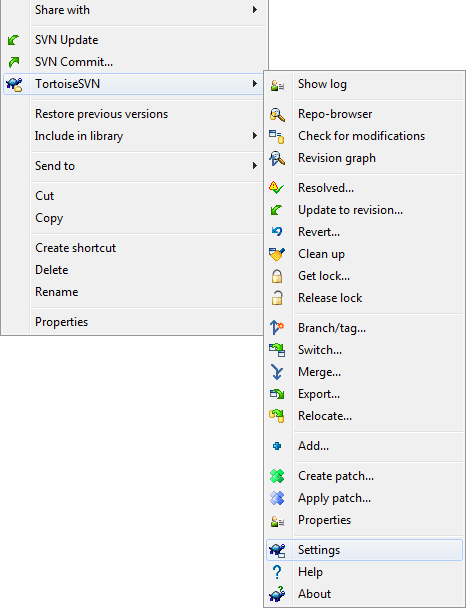
\includegraphics[width=0.70\textwidth]{figures/tortoise_svn_accessing_settings.png}
	\caption{Getting to the TortoiseSVN settings.}
	\label{fig:tortoise_svn_accessing_settings}
\end{figure}
\clearpage

\noindent The settings window will look something like this:

\begin{figure}[h!]
	\centering
		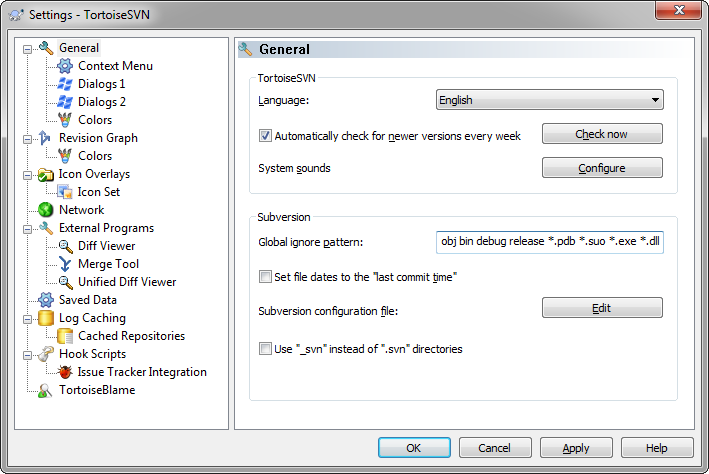
\includegraphics[width=0.90\textwidth]{figures/tortoise_svn_ignore_patterns.png}
	\caption{The TortoiseSVN settings window with the proper ignore pattern.}
	\label{fig:tortoise_svn_ignore_patterns}
\end{figure}

\noindent Then in the \textit{Global ignore pattern} field, please enter the following text:

\begin{center}
\textit{obj bin debug release *.pdb *.suo *.exe *.dll *.aux *.dvi *.log *.bak *.bbl *.blg *.user}
\end{center}

You are free to also leave in any default pattern text or to write your own additions; this pattern serves simply to tell TortoiseSVN what kinds of files to ignore. You can now click \textit{OK} to save your settings and close the window.
\clearpage

\subsection{Committing your changes}
\label{CommitingYourChanges}

Once you start writing code and developing your plugin, you should check your work into the project repository. If you are reading this document in sequence, you are probably not ready to do this, but while we are on the topic of SVN we will describe the process. To upload your changes, right-click on a directory within the working files that contains your changes and select \textit{SVN Commit} from the context menu:

\begin{figure}[h!]
	\centering
		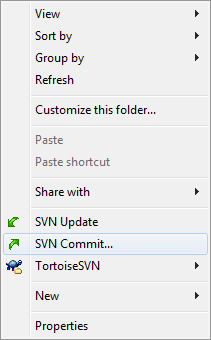
\includegraphics[width=0.40\textwidth]{figures/tortoise_svn_commit.png}
	\caption{Selecting \textit{SVN Commit} from the context menu.}
	\label{fig:tortoise_svn_commit}
\end{figure}
\clearpage

When you commit your code, you must enter a comment to describe what you have changed. \textit{Meaningful descriptions} will help other developers to comprehend your updates. You can also select exactly which files you want to check in. The ignore pattern that we recommended should prevent most undesirable files from being in the list, but double-check to make sure everything you want to upload is included but nothing more. In general, you should never check in compiled and automatically generated files. For example, do not check in the entire \texttt{bin\textbackslash} and \texttt{obj\textbackslash} directories that Visual Studio generates. The server will reject your commits if you try to do so. You should commit your sources to our SVN repository as often as you can, even when it's not finished or when there are bugs. However your committed code should not break anything existing, so please make sure the public solution successfully still compiles and runs.

\begin{figure}[h!]
	\centering
		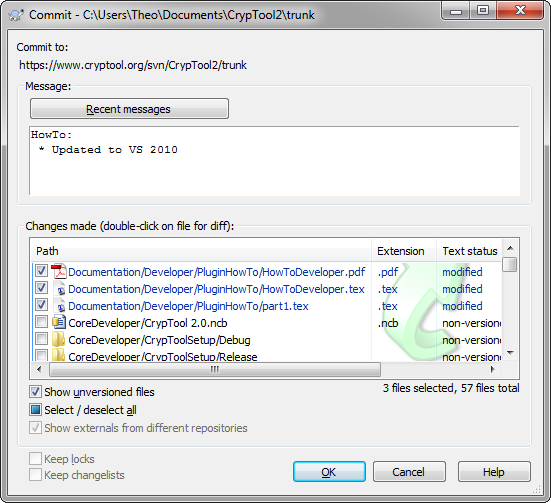
\includegraphics[width=0.70\textwidth]{figures/tortoise_svn_commit_window.png}
	\caption{Providing comments for a commit.}
	\label{fig:tortoise_svn_commit2}
\end{figure}

You can use the SVN comments to link to your changes to a particular issue or bug ticket on the CrypTool 2 development wiki. (The list of active tickets can be found \href{https://www.cryptool.org/trac/CrypTool2/report/1}{here}.) The following commands are supported (note that there are multiple variations of each command that are functionally identical):

\begin{center}
\fbox{\parbox{15cm}
{
\texttt{closes, fixes:}

The specified ticket will be closed and the contents of this commit message will be added to its notes.\\

\texttt{references, refs, addresses, re:}

The contents of this commit message will be added to the specified ticket's notes, but the status will be left unaltered.
}}
\end{center}
\clearpage

You can apply the commands to multiple tickets simultaneously. The command syntax is as follows (again note that there are multiple variations that are functionally identical):

\begin{center}
\fbox{\parbox{15cm}
{\tt
command \#1\\
command \#1, \#2\\
command \#1 \& \#2\\
command \#1 and \#2
}}
\end{center}

You can also use more than one command in a message if necessary. For example, if you want to close tickets \#10 and \#12, and add a note to \#17, you could type the following:

\begin{center}
\fbox{\parbox{15cm}
{\tt
Changed blah and foo to do this or that.\ Fixes \#10 and \#12, and refs \#17.
}}
\end{center}

The comments can also be used to override the ignore pattern that the server is designed to block. However, please do not do this unless you are absolutely sure that you know what you are doing. If you are, you must use the \textit{override-bad-extension} command and provide an explicit list of the file and directory names that you want to upload that need to override the ignore pattern. For example, if you want to check in a library file named \textit{someLib.dll}, you must write something like the following:

\begin{center}
\fbox{\parbox{15cm}
{\tt
This library is referenced by project xy.\\\\
override-bad-extension:\ someLib.dll
}}
\end{center}

Note that any text after the colon and the whitespace will be treated as the file name. Therefore, do not use quotation marks and do not write any text after the file name.

\section{Compiling the sources with Visual Studio 2010}
\label{CompilingTheSourcesVS}

By this point you should have checked out a copy of the entire CrypTool~2 repository. Compiling is pretty easy; just go to the \texttt{trunk\textbackslash} directory and open the \textbf{\textit{CrypTool 2.0.sln}} Visual Studio solution. The Visual Studio IDE should open with all the working plugin components nicely arranged. If you are now starting Visual Studio for the first time, you will have to choose your settings. Just select either \textit{most common} or \textit{C\#} --- you can change this at any time later. On the right side is the project explorer, where you can see all the subprojects included in the solution. Look for the project \textbf{\textit{CrypStartup}} there and make sure it is selected as startup project (right-click on it and select \textit{Set as StartUp Project} from the context menu). Next, go to the menu bar and make sure the target platform is set correctly (Figure~\ref{fig:vs_menubar_x86}). If your operating system is a 32 bit installation, you have to select \textbf{x86}. If you have a 64 bit operating system, you may use one of both, x64 or x86. If in doubt, select x86. Then click \textit{Build $\rightarrow$ Build Solution} in the menubar to start the build process.

\begin{figure}[htbp]
	\centering
		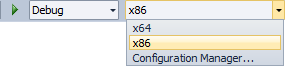
\includegraphics{figures/vs_menubar_x86.png}
	\caption{Selecting x86 as target platform.}
	\label{fig:vs_menubar_x86}
\end{figure}
\clearpage

You may have to wait a while for the program to compile. Once it is finished, select \textit{Debug $\rightarrow$ Start Debugging}. CrypTool 2 should now start for the first time with your own compiled code. Presumably you have not changed anything yet, but you now have your own build of all the components (with the exception of \textit{CrypWin} and \textit{AnotherEditor}, since they are available only as binaries). If the program does not compile or start correctly, please consult our \href{https://www.cryptool.org/trac/CrypTool2/wiki/FAQ}{FAQ} and let us know if you found a bug.

If you are a \textbf{core developer}, hence somebody who can also compile CrypWin and AnotherEditor, you can use the \textbf{\textit{CrypTool 2.0.sln}} solution from the \texttt{CoreDeveloper\textbackslash} directory (which will \textit{not} be visible to you if you are not a core developer). As a core developer, be aware that when you compile, you \textbf{change the \textit{CrypWin.exe}} that is visible to everybody else. Thus, when committing to the repository, please make sure you \textit{really} want to check in a new binary.

\section{Compiling the sources with Visual C\# 2010 Express}
\label{CompilingTheSourcesExpress}

With Visual C\# Express the build process is basically the same as with Visual Studio. When opening the solution file, you will receive two error messages. The first is because Visual C\# does not support solution folders and shows all plugin projects as a flat list in the solution explorer. However this is only a visual defect. The second error message is, because Visual C\# does not support unit tests and thus is not able to load the project \textit{DevTestMethods}. Again, this does not interfere with opening, writing, compiling, running or debugging plugins.

\section{Downloading the plugin template}
\label{DownloadingThePluginTemplate}

Before you can start implementing a new plugin, you will have to download the CrypTool~2 plugin template. The template is located at the CrypTool 2 website at \url{http://www.cryptool2.vs.uni-due.de/index.php?page=33&lm=3}. Save the template zip file in your documents folder in the subdirectory \texttt{Visual Studio 2010\textbackslash{}Templates\textbackslash{}Project Templates\textbackslash{}} (applies to both, Visual Studio and Visual C\# Express). Do not unpack the zip file.
